Let $ABC$ be a triangle with circumcircle $k$. Let $A_1,B_1$ and $C_1$ be points on the interior of the sides $BC,CA$ and $AB$ respectively. Let $X$ be a point on $k$ and denote by $Y$ the second intersection of the circumcircles of $BC_1X$ and $CB_1X$. Define the points $P$ and $Q$ to be the intersections of $BY$ with $B_1A_1$ and $CY$ with $C_1A_1$, respectively. Prove that $A$ lies on the line $PQ$.

\textbf{Solution:} We first show that the points $B_1$, $Y$ and $C_1$ are collinear. Let $\angle B_1 Y X = \alpha$. Using the cyclic quadrilateral $B_1YXC$ we have $\angle X C B_1 = 180- \alpha$. Similarly using the cyclic quadrilaterals $CABX$ and $C_1BXY$, we arrive at $\angle C_1 B X = \alpha$ and $\angle XY C_1 = 180- \alpha$. So indeed $B_1$, $Y$ and $C_1$ are collinear. 

\begin{figure}[h!]
    \centering
    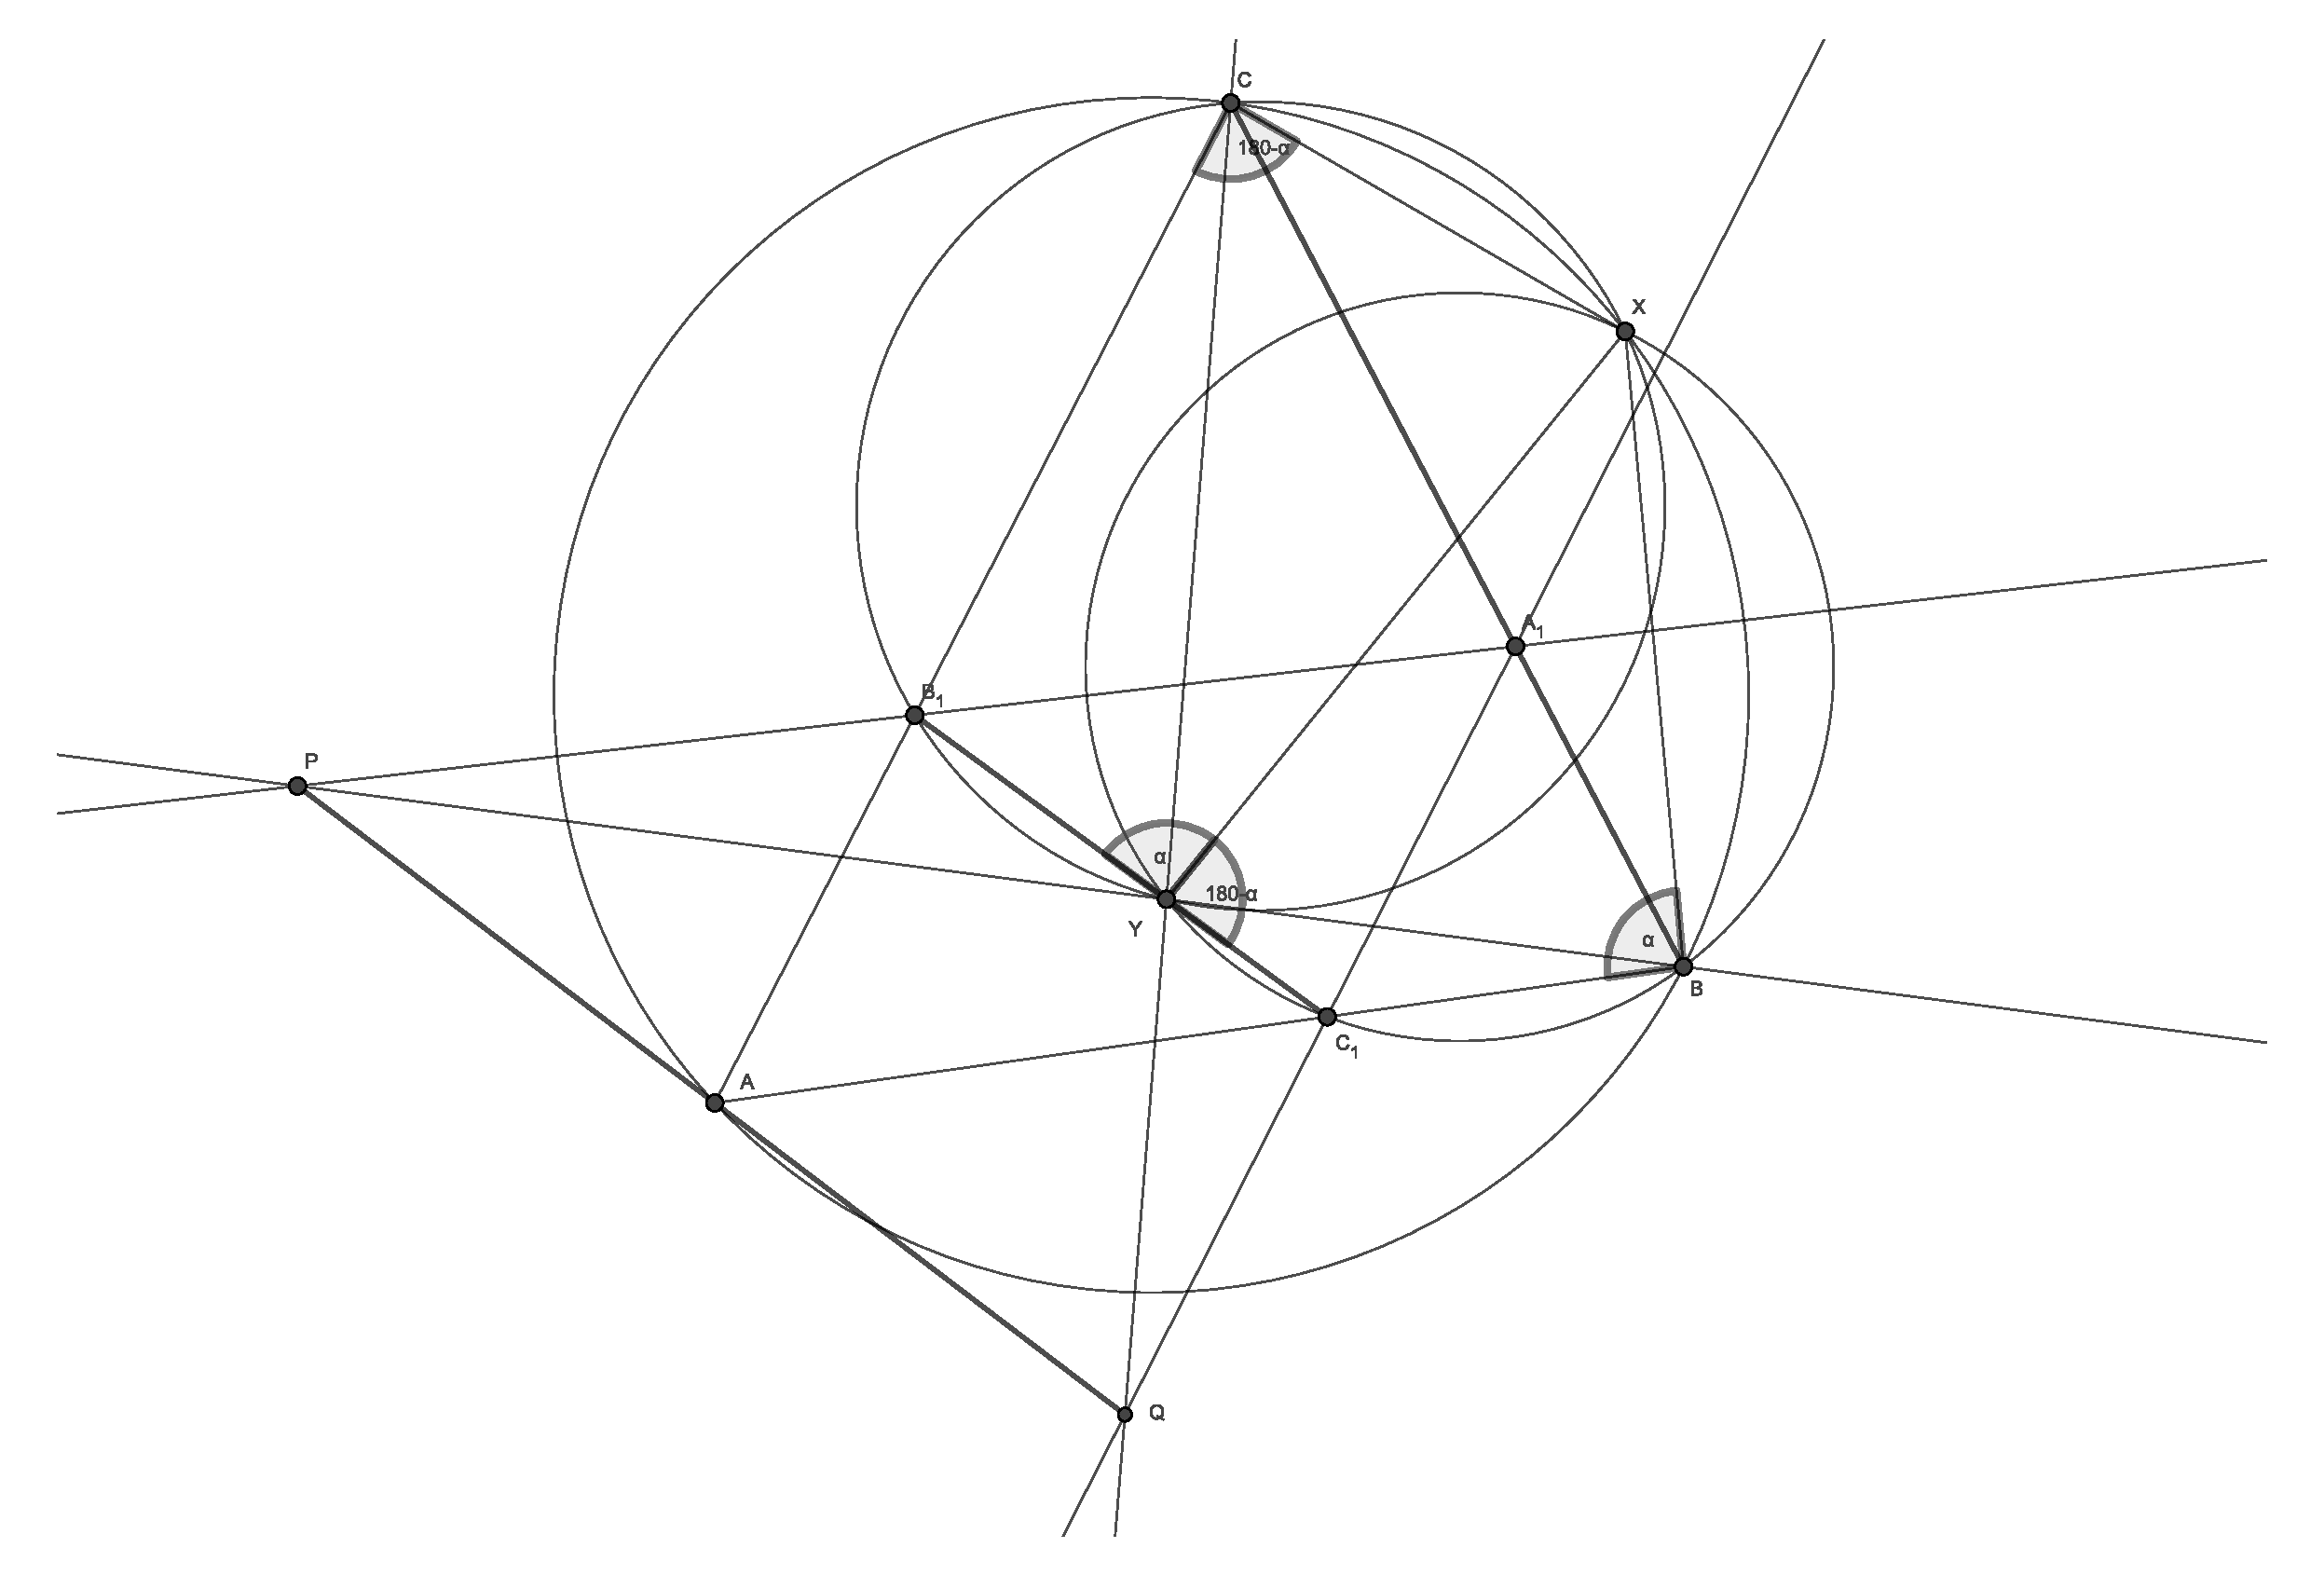
\includegraphics[width = 0.8\textwidth]{solutions/s10_solpic.pdf}
    \caption{Solution of problem 10}
\end{figure}

 Using Pappus theorem on the two sets of collinear points $\{B_1, Y, C_1\}$ and $\{B, A_1, C\}$, we can now proof that $P$, $Q$ and $A$ are also collinear. 


\textbf{Marking Scheme}
\begin{itemize}
    \item 1P : Guessing that $B_1$, $Y$ and $C_1$ are collinear.
    \item 3P : Proving it.
    \item 3P:  Use Pappus.
\end{itemize}

1P can be awarded for someone using Pappus with the correct lines but a wrong order of the points
